\chapter{Introducción}

\section{Antecedentes y motivación}

\begin{figure}
    \centering
    \begin{subfigure}[c]{0.45\textwidth}
        \centering
        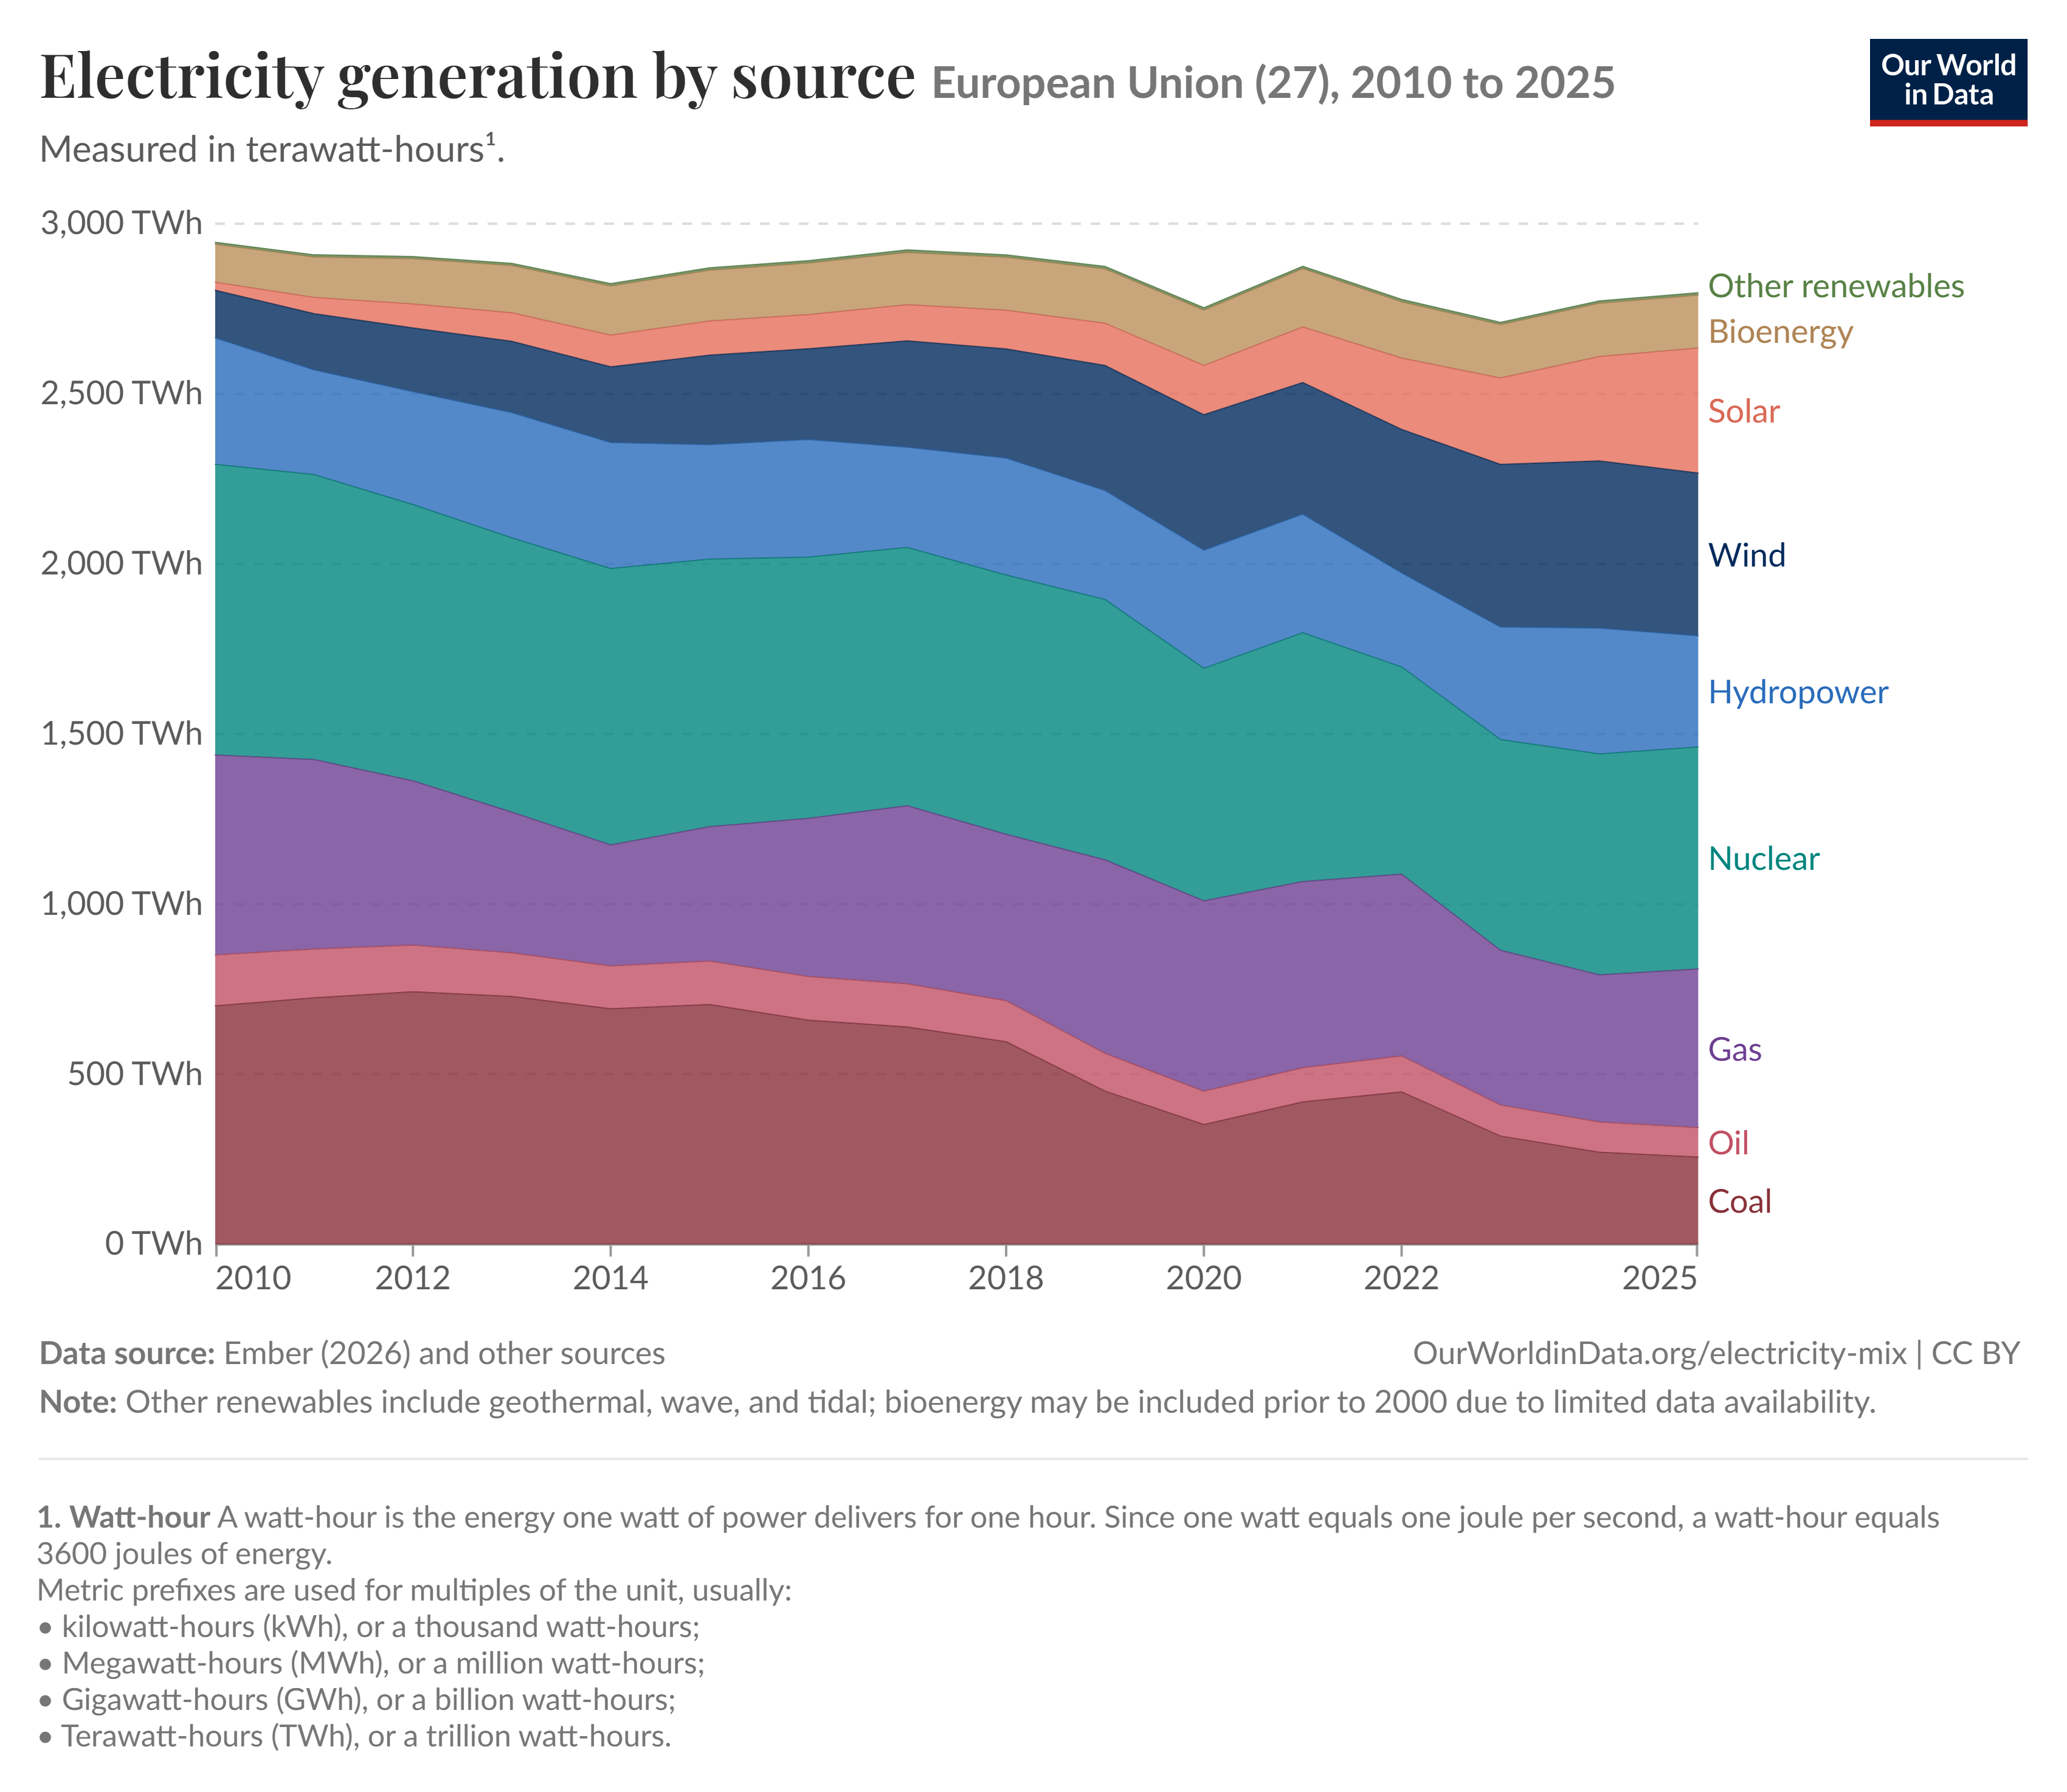
\includegraphics[width =  \textwidth]{Imagenes/electricity-mix.png}
        \caption{}
    \end{subfigure}
    \hfill
    \begin{subfigure}[c]{0.45\textwidth}
        \centering
        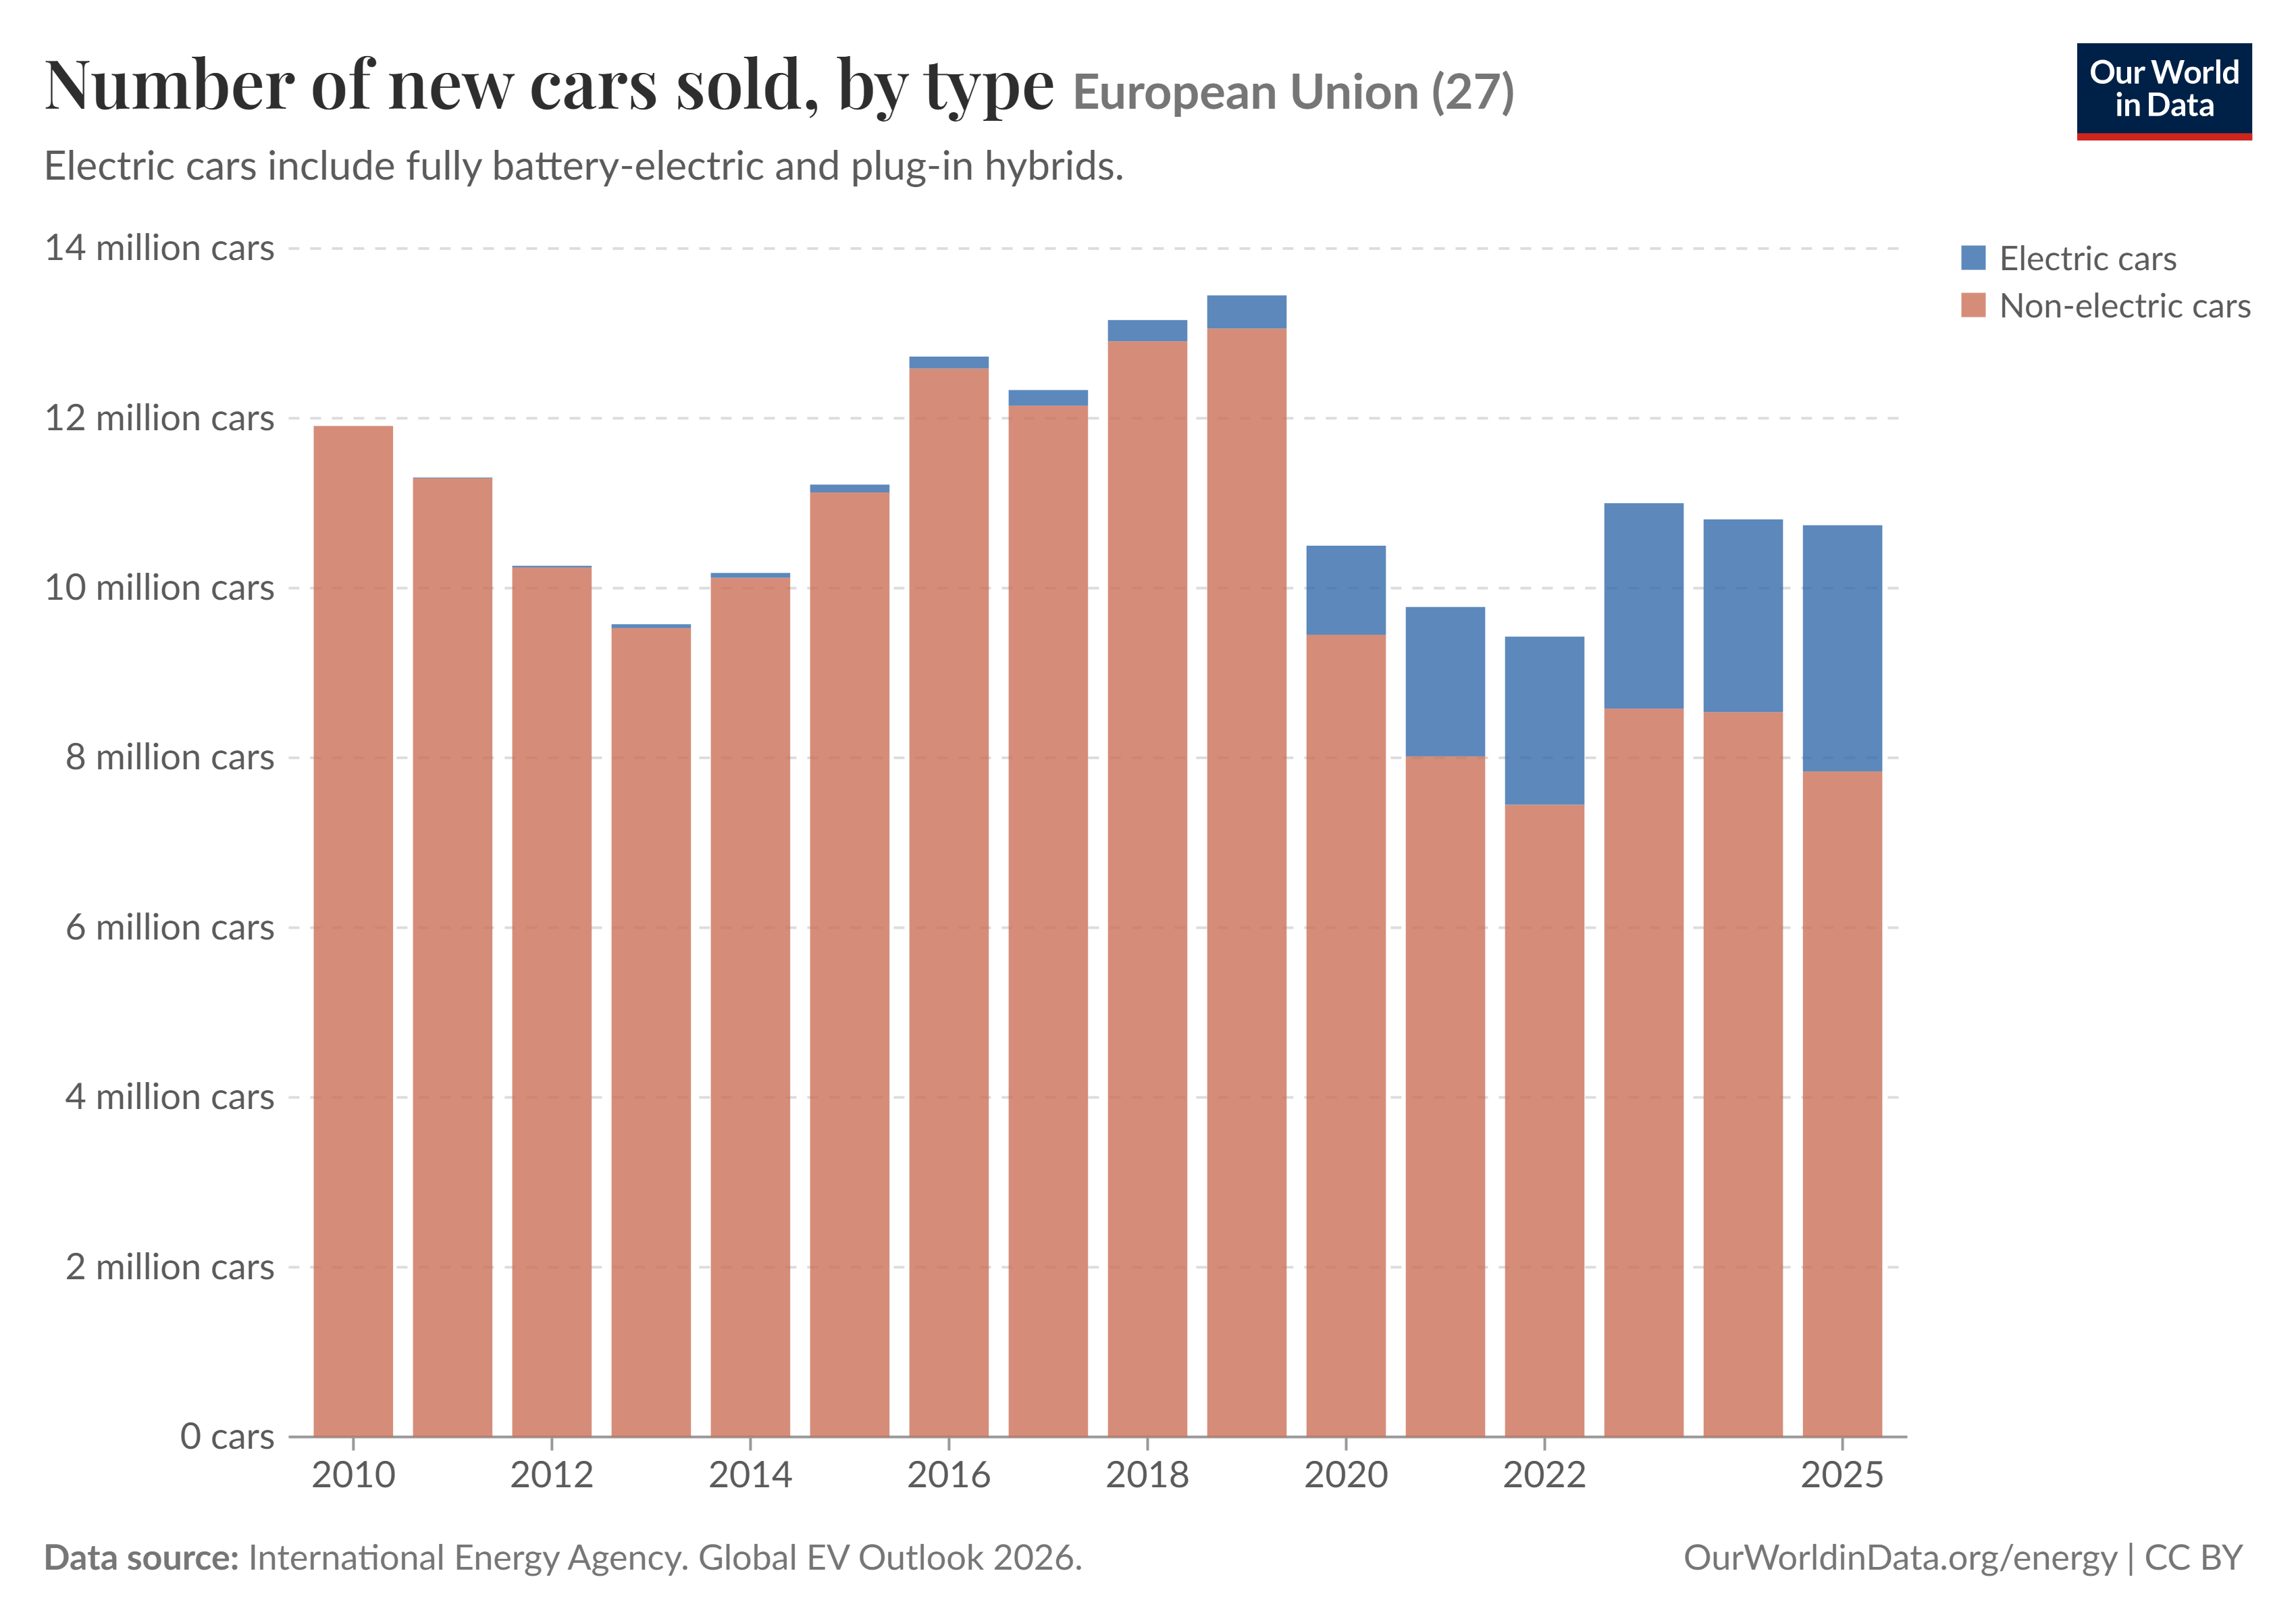
\includegraphics[width =  \textwidth]{Imagenes/car-sales.png}
        \caption{}
    \end{subfigure}
    \caption{\cite{Data2024}}
    \label{fig: Evolucion Union Europea}
\end{figure}

La transición hacia un modelo energético más sostenibles y a la descarbonicación de la economía son dos de los mayores retos a los que se enfrenta la sociedad actual. Como se observa en la figura \ref{fig: Evolucion Union Europea}, en la Unión Europea se ha producido un cambio visible en los últimos años tanto en la presencia de energías renovables en el mix energético como en la venta de vehículos eléctricos.

Ente 2010 y 2025, las energías renovables han ido incrementando su importancia frente a las formas de generación de energía tradicionales, disminuyendo así la depencia de combustibles fósiles. Siguiendo esta tendencia, la venta de vehículos eléctricos en este tiempo ha aumentado considerablemente frente a la de los vehículos de combustión.

El pilar fundamental que hace posible estos cambios son los avances en la electrónica de potencia, más concretamente, en los inversores. En el caso de la generación de energía, los inversores son esenciales para convertir la corrinte continua (DC) que genera por ejemplo los paneles fotovoltáicos, en energía inyectable a la red. Por otro lado, en los vehículos eléctricos, los inversores son los encargados de convertir la energía almacenada en las baterías en la corriente alterna (AC) que necesitan los motores eléctricos.

\section{Objetivos del trabajo}

\section{Metodología y estructura de la memoria}
